\section{Platform}
\label{sec:platform}
In this system overview, the platform along with the electronics and its software is described to aid in understanding the physical interconnections that exist between the modules.

The system consists of a wide range of modules which may be sensors or actuators. These modules are connected to a \ac{LLI} and \ac{HLI} computing device. The \ac{LLI} is a microcontroller which takes care of the basic functions of the platform such as communicating with basic sensors and actuators. The software for this is embedded and written in C for the avr-gcc compiler.

The \ac{HLI} is a x86 compatible computer of some sort that is able to run the higher abstraction layer code written in Python. This code implements the onboard generation of waypoints from map data to calculate the desired heading and speed for the vessel. It also implements the state space model and calculates propeller speeds and in turn sends these to the \ac{LLI}.

Some modules that are connected to the \ac{LLI} are not handled by the \ac{LLI} itself, but instead it forwards the data to the \ac{HLI} which uses it for the control algorithm. A illustration of this can be seen on figure~\vref{fig:vessel-block-overview}.

\begin{figure}[htbp]
	\centering
	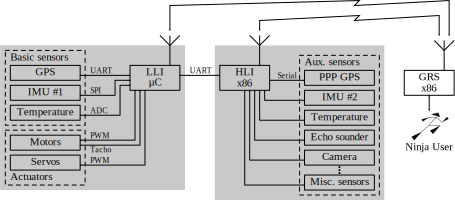
\includegraphics[width=\textwidth]{img/vessel-block-overview-electrical}
	\caption{Overview of electrical interconnections between \ac{LLI} and \ac{HLI} together with periphal modules.}
	\label{fig:vessel-block-overview-electrical}
\end{figure}
